% Options for packages loaded elsewhere
\PassOptionsToPackage{unicode}{hyperref}
\PassOptionsToPackage{hyphens}{url}
\PassOptionsToPackage{dvipsnames,svgnames,x11names}{xcolor}
%
\documentclass[
]{report}

\usepackage{amsmath,amssymb}
\usepackage{iftex}
\ifPDFTeX
  \usepackage[T1]{fontenc}
  \usepackage[utf8]{inputenc}
  \usepackage{textcomp} % provide euro and other symbols
\else % if luatex or xetex
  \usepackage{unicode-math}
  \defaultfontfeatures{Scale=MatchLowercase}
  \defaultfontfeatures[\rmfamily]{Ligatures=TeX,Scale=1}
\fi
\usepackage{lmodern}
\ifPDFTeX\else  
    % xetex/luatex font selection
\fi
% Use upquote if available, for straight quotes in verbatim environments
\IfFileExists{upquote.sty}{\usepackage{upquote}}{}
\IfFileExists{microtype.sty}{% use microtype if available
  \usepackage[]{microtype}
  \UseMicrotypeSet[protrusion]{basicmath} % disable protrusion for tt fonts
}{}
\makeatletter
\@ifundefined{KOMAClassName}{% if non-KOMA class
  \IfFileExists{parskip.sty}{%
    \usepackage{parskip}
  }{% else
    \setlength{\parindent}{0pt}
    \setlength{\parskip}{6pt plus 2pt minus 1pt}}
}{% if KOMA class
  \KOMAoptions{parskip=half}}
\makeatother
\usepackage{xcolor}
\setlength{\emergencystretch}{3em} % prevent overfull lines
\setcounter{secnumdepth}{-\maxdimen} % remove section numbering
% Make \paragraph and \subparagraph free-standing
\ifx\paragraph\undefined\else
  \let\oldparagraph\paragraph
  \renewcommand{\paragraph}[1]{\oldparagraph{#1}\mbox{}}
\fi
\ifx\subparagraph\undefined\else
  \let\oldsubparagraph\subparagraph
  \renewcommand{\subparagraph}[1]{\oldsubparagraph{#1}\mbox{}}
\fi

\usepackage{color}
\usepackage{fancyvrb}
\newcommand{\VerbBar}{|}
\newcommand{\VERB}{\Verb[commandchars=\\\{\}]}
\DefineVerbatimEnvironment{Highlighting}{Verbatim}{commandchars=\\\{\}}
% Add ',fontsize=\small' for more characters per line
\usepackage{framed}
\definecolor{shadecolor}{RGB}{241,243,245}
\newenvironment{Shaded}{\begin{snugshade}}{\end{snugshade}}
\newcommand{\AlertTok}[1]{\textcolor[rgb]{0.68,0.00,0.00}{#1}}
\newcommand{\AnnotationTok}[1]{\textcolor[rgb]{0.37,0.37,0.37}{#1}}
\newcommand{\AttributeTok}[1]{\textcolor[rgb]{0.40,0.45,0.13}{#1}}
\newcommand{\BaseNTok}[1]{\textcolor[rgb]{0.68,0.00,0.00}{#1}}
\newcommand{\BuiltInTok}[1]{\textcolor[rgb]{0.00,0.23,0.31}{#1}}
\newcommand{\CharTok}[1]{\textcolor[rgb]{0.13,0.47,0.30}{#1}}
\newcommand{\CommentTok}[1]{\textcolor[rgb]{0.37,0.37,0.37}{#1}}
\newcommand{\CommentVarTok}[1]{\textcolor[rgb]{0.37,0.37,0.37}{\textit{#1}}}
\newcommand{\ConstantTok}[1]{\textcolor[rgb]{0.56,0.35,0.01}{#1}}
\newcommand{\ControlFlowTok}[1]{\textcolor[rgb]{0.00,0.23,0.31}{#1}}
\newcommand{\DataTypeTok}[1]{\textcolor[rgb]{0.68,0.00,0.00}{#1}}
\newcommand{\DecValTok}[1]{\textcolor[rgb]{0.68,0.00,0.00}{#1}}
\newcommand{\DocumentationTok}[1]{\textcolor[rgb]{0.37,0.37,0.37}{\textit{#1}}}
\newcommand{\ErrorTok}[1]{\textcolor[rgb]{0.68,0.00,0.00}{#1}}
\newcommand{\ExtensionTok}[1]{\textcolor[rgb]{0.00,0.23,0.31}{#1}}
\newcommand{\FloatTok}[1]{\textcolor[rgb]{0.68,0.00,0.00}{#1}}
\newcommand{\FunctionTok}[1]{\textcolor[rgb]{0.28,0.35,0.67}{#1}}
\newcommand{\ImportTok}[1]{\textcolor[rgb]{0.00,0.46,0.62}{#1}}
\newcommand{\InformationTok}[1]{\textcolor[rgb]{0.37,0.37,0.37}{#1}}
\newcommand{\KeywordTok}[1]{\textcolor[rgb]{0.00,0.23,0.31}{#1}}
\newcommand{\NormalTok}[1]{\textcolor[rgb]{0.00,0.23,0.31}{#1}}
\newcommand{\OperatorTok}[1]{\textcolor[rgb]{0.37,0.37,0.37}{#1}}
\newcommand{\OtherTok}[1]{\textcolor[rgb]{0.00,0.23,0.31}{#1}}
\newcommand{\PreprocessorTok}[1]{\textcolor[rgb]{0.68,0.00,0.00}{#1}}
\newcommand{\RegionMarkerTok}[1]{\textcolor[rgb]{0.00,0.23,0.31}{#1}}
\newcommand{\SpecialCharTok}[1]{\textcolor[rgb]{0.37,0.37,0.37}{#1}}
\newcommand{\SpecialStringTok}[1]{\textcolor[rgb]{0.13,0.47,0.30}{#1}}
\newcommand{\StringTok}[1]{\textcolor[rgb]{0.13,0.47,0.30}{#1}}
\newcommand{\VariableTok}[1]{\textcolor[rgb]{0.07,0.07,0.07}{#1}}
\newcommand{\VerbatimStringTok}[1]{\textcolor[rgb]{0.13,0.47,0.30}{#1}}
\newcommand{\WarningTok}[1]{\textcolor[rgb]{0.37,0.37,0.37}{\textit{#1}}}

\providecommand{\tightlist}{%
  \setlength{\itemsep}{0pt}\setlength{\parskip}{0pt}}\usepackage{longtable,booktabs,array}
\usepackage{calc} % for calculating minipage widths
% Correct order of tables after \paragraph or \subparagraph
\usepackage{etoolbox}
\makeatletter
\patchcmd\longtable{\par}{\if@noskipsec\mbox{}\fi\par}{}{}
\makeatother
% Allow footnotes in longtable head/foot
\IfFileExists{footnotehyper.sty}{\usepackage{footnotehyper}}{\usepackage{footnote}}
\makesavenoteenv{longtable}
\usepackage{graphicx}
\makeatletter
\def\maxwidth{\ifdim\Gin@nat@width>\linewidth\linewidth\else\Gin@nat@width\fi}
\def\maxheight{\ifdim\Gin@nat@height>\textheight\textheight\else\Gin@nat@height\fi}
\makeatother
% Scale images if necessary, so that they will not overflow the page
% margins by default, and it is still possible to overwrite the defaults
% using explicit options in \includegraphics[width, height, ...]{}
\setkeys{Gin}{width=\maxwidth,height=\maxheight,keepaspectratio}
% Set default figure placement to htbp
\makeatletter
\def\fps@figure{htbp}
\makeatother

\makeatletter
\makeatother
\makeatletter
\makeatother
\makeatletter
\@ifpackageloaded{caption}{}{\usepackage{caption}}
\AtBeginDocument{%
\ifdefined\contentsname
  \renewcommand*\contentsname{Table of contents}
\else
  \newcommand\contentsname{Table of contents}
\fi
\ifdefined\listfigurename
  \renewcommand*\listfigurename{List of Figures}
\else
  \newcommand\listfigurename{List of Figures}
\fi
\ifdefined\listtablename
  \renewcommand*\listtablename{List of Tables}
\else
  \newcommand\listtablename{List of Tables}
\fi
\ifdefined\figurename
  \renewcommand*\figurename{Figure}
\else
  \newcommand\figurename{Figure}
\fi
\ifdefined\tablename
  \renewcommand*\tablename{Table}
\else
  \newcommand\tablename{Table}
\fi
}
\@ifpackageloaded{float}{}{\usepackage{float}}
\floatstyle{ruled}
\@ifundefined{c@chapter}{\newfloat{codelisting}{h}{lop}}{\newfloat{codelisting}{h}{lop}[chapter]}
\floatname{codelisting}{Listing}
\newcommand*\listoflistings{\listof{codelisting}{List of Listings}}
\makeatother
\makeatletter
\@ifpackageloaded{caption}{}{\usepackage{caption}}
\@ifpackageloaded{subcaption}{}{\usepackage{subcaption}}
\makeatother
\makeatletter
\@ifpackageloaded{tcolorbox}{}{\usepackage[skins,breakable]{tcolorbox}}
\makeatother
\makeatletter
\@ifundefined{shadecolor}{\definecolor{shadecolor}{rgb}{.97, .97, .97}}
\makeatother
\makeatletter
\makeatother
\makeatletter
\makeatother
\ifLuaTeX
  \usepackage{selnolig}  % disable illegal ligatures
\fi
\IfFileExists{bookmark.sty}{\usepackage{bookmark}}{\usepackage{hyperref}}
\IfFileExists{xurl.sty}{\usepackage{xurl}}{} % add URL line breaks if available
\urlstyle{same} % disable monospaced font for URLs
\hypersetup{
  pdftitle={EPIDEMIOLOGY OF MULTI-DRUG RESISTANT TB USING ISOLATES SENT TO THE NATIONAL TUBERCULOSIS REFERENCE LABORARY (2015-2016)},
  colorlinks=true,
  linkcolor={blue},
  filecolor={Maroon},
  citecolor={Blue},
  urlcolor={Blue},
  pdfcreator={LaTeX via pandoc}}

\title{EPIDEMIOLOGY OF MULTI-DRUG RESISTANT TB USING ISOLATES SENT TO
THE NATIONAL TUBERCULOSIS REFERENCE LABORARY (2015-2016)}
\author{}
\date{}

\begin{document}
\maketitle
\ifdefined\Shaded\renewenvironment{Shaded}{\begin{tcolorbox}[borderline west={3pt}{0pt}{shadecolor}, interior hidden, breakable, enhanced, frame hidden, sharp corners, boxrule=0pt]}{\end{tcolorbox}}\fi

\hypertarget{methods}{%
\chapter{METHODS}\label{methods}}

\begin{Shaded}
\begin{Highlighting}[]
\FunctionTok{library}\NormalTok{(}\StringTok{\textquotesingle{}ggflowchart\textquotesingle{}}\NormalTok{)}
\NormalTok{flow\_chart }\OtherTok{\textless{}{-}}\NormalTok{ tibble}\SpecialCharTok{::}\FunctionTok{tibble}\NormalTok{(}\AttributeTok{from =} \FunctionTok{c}\NormalTok{(}\StringTok{"Total TB+ Entries recieved }
\StringTok{  8308"}\NormalTok{, }\StringTok{"Total TB+ Entries recieved }
\StringTok{  8308"}\NormalTok{, }\StringTok{"Entries after removing null values}
\StringTok{  2621"}\NormalTok{, }\StringTok{"Entries after removing null values}
\StringTok{  2621"}\NormalTok{, }\StringTok{"Null entries removed}
\StringTok{  2621"}\NormalTok{),}
                             \AttributeTok{to=} \FunctionTok{c}\NormalTok{(}\StringTok{"Entries after removing null values}
\StringTok{  2621"}\NormalTok{,}\StringTok{"Entries removed }
\StringTok{  5682"}\NormalTok{, }\StringTok{"Entries after removing Non{-}MDR}
\StringTok{  143}
\StringTok{  "}\NormalTok{, }\StringTok{"Null entries removed}
\StringTok{  2621"}\NormalTok{, }\StringTok{"MDR entries analyzed}
\StringTok{  143"}\NormalTok{))}
\FunctionTok{ggflowchart}\NormalTok{(flow\_chart, }\AttributeTok{colour =} \StringTok{\textquotesingle{}cyan\textquotesingle{}}\NormalTok{, }\AttributeTok{family =} \StringTok{\textquotesingle{}serif\textquotesingle{}}\NormalTok{, }\AttributeTok{x\_nudge =} \FloatTok{0.45}\NormalTok{)}
\end{Highlighting}
\end{Shaded}

\begin{figure}[H]

{\centering 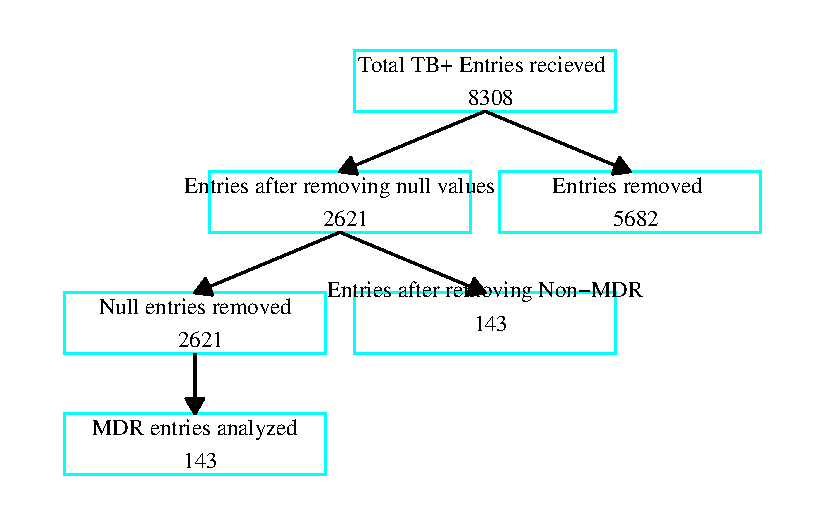
\includegraphics{MDR_TB_files/figure-pdf/unnamed-chunk-1-1.pdf}

}

\end{figure}

\hypertarget{r-packages-used}{%
\section{R Packages used}\label{r-packages-used}}

\begin{Shaded}
\begin{Highlighting}[]
\CommentTok{\#\textbackslash{} label: load{-}packages}
\FunctionTok{suppressPackageStartupMessages}\NormalTok{(}\FunctionTok{library}\NormalTok{(}\StringTok{\textquotesingle{}tidyverse\textquotesingle{}}\NormalTok{))}

\CommentTok{\#install.packages(\textquotesingle{}plotly\textquotesingle{})}

\CommentTok{\#install.packages(\textquotesingle{}ggmap\textquotesingle{})}

\CommentTok{\#install.packages(\textquotesingle{}forcats\textquotesingle{})}
\FunctionTok{suppressPackageStartupMessages}\NormalTok{(}\FunctionTok{library}\NormalTok{(}\StringTok{\textquotesingle{}ggmap\textquotesingle{}}\NormalTok{))}
\FunctionTok{suppressPackageStartupMessages}\NormalTok{(}\FunctionTok{library}\NormalTok{(}\StringTok{\textquotesingle{}plotly\textquotesingle{}}\NormalTok{))}
\FunctionTok{suppressPackageStartupMessages}\NormalTok{(}\FunctionTok{library}\NormalTok{(}\StringTok{\textquotesingle{}ggdist\textquotesingle{}}\NormalTok{))}
\FunctionTok{suppressPackageStartupMessages}\NormalTok{(}\FunctionTok{library}\NormalTok{(}\StringTok{\textquotesingle{}ggmap\textquotesingle{}}\NormalTok{))}
\end{Highlighting}
\end{Shaded}

\hypertarget{functions}{%
\chapter{FUNCTIONS}\label{functions}}

\hypertarget{fishers-function}{%
\section{Fisher's function}\label{fishers-function}}

\begin{Shaded}
\begin{Highlighting}[]
\NormalTok{Fishersfn }\OtherTok{\textless{}{-}} \ControlFlowTok{function}\NormalTok{(df, var1, var2)\{}

\NormalTok{  contingency\_table }\OtherTok{\textless{}{-}} \FunctionTok{table}\NormalTok{(df[[var1]], df[[var2]])}

\NormalTok{  fisherExact }\OtherTok{\textless{}{-}} \FunctionTok{fisher.test}\NormalTok{(contingency\_table)}

  \FunctionTok{return}\NormalTok{ (fisherExact)}

\NormalTok{\}}
\end{Highlighting}
\end{Shaded}

\hypertarget{getting-percentages}{%
\section{Getting percentages}\label{getting-percentages}}

\begin{Shaded}
\begin{Highlighting}[]
\NormalTok{pcts }\OtherTok{\textless{}{-}} \ControlFlowTok{function}\NormalTok{(df, var\_to\_group\_by) \{}

\NormalTok{  results }\OtherTok{\textless{}{-}}\NormalTok{ df }\SpecialCharTok{\%\textgreater{}\%}

    \FunctionTok{group\_by\_at}\NormalTok{(}\FunctionTok{vars}\NormalTok{(\{\{ var\_to\_group\_by \}\})) }\SpecialCharTok{\%\textgreater{}\%}

    \FunctionTok{summarise}\NormalTok{(}\AttributeTok{counts =} \FunctionTok{n}\NormalTok{()) }\SpecialCharTok{\%\textgreater{}\%}

    \FunctionTok{mutate}\NormalTok{(}\AttributeTok{Percentages =}\NormalTok{ counts}\SpecialCharTok{/}\FunctionTok{sum}\NormalTok{(counts)}\SpecialCharTok{*}\DecValTok{100}\NormalTok{)}

  

  \FunctionTok{return}\NormalTok{(results)}

\NormalTok{\}}
\end{Highlighting}
\end{Shaded}

Reading the file

\begin{Shaded}
\begin{Highlighting}[]
\NormalTok{mdr\_tb\_df }\OtherTok{\textless{}{-}} \FunctionTok{read.csv}\NormalTok{(}\StringTok{\textquotesingle{}mdr\_tbv4.csv\textquotesingle{}}\NormalTok{)}
\end{Highlighting}
\end{Shaded}

Creating a new column to define MDR\_TYPE

\begin{Shaded}
\begin{Highlighting}[]
\NormalTok{mdr\_tb\_df}\SpecialCharTok{$}\NormalTok{MDR\_TYPE }\OtherTok{\textless{}{-}} \ConstantTok{NA}
\end{Highlighting}
\end{Shaded}

Here I have defined Rpob + katg as MDRKR (MDR KatG and RpoB), as well as
those that are rpob + katg + inha

\begin{Shaded}
\begin{Highlighting}[]
\NormalTok{mdr\_tb\_dfv1 }\OtherTok{\textless{}{-}}\NormalTok{ mdr\_tb\_df}\SpecialCharTok{$}\NormalTok{MDR\_TYPE[mdr\_tb\_df}\SpecialCharTok{$}\NormalTok{RpoB }\SpecialCharTok{==} \StringTok{\textquotesingle{}Resistant\textquotesingle{}} \SpecialCharTok{\&}\NormalTok{ mdr\_tb\_df}\SpecialCharTok{$}\NormalTok{KatG }\SpecialCharTok{==} \StringTok{\textquotesingle{}Resistant\textquotesingle{}}\NormalTok{] }\OtherTok{\textless{}{-}} \StringTok{\textquotesingle{}MDRKR\textquotesingle{}}

\NormalTok{mdr\_tb\_df}\SpecialCharTok{$}\NormalTok{MDR\_TYPE[mdr\_tb\_df}\SpecialCharTok{$}\NormalTok{RpoB }\SpecialCharTok{==} \StringTok{\textquotesingle{}Resistant\textquotesingle{}} \SpecialCharTok{\&}\NormalTok{ mdr\_tb\_df}\SpecialCharTok{$}\NormalTok{KatG }\SpecialCharTok{!=} \StringTok{\textquotesingle{}Resistant\textquotesingle{}} \SpecialCharTok{\&}\NormalTok{ mdr\_tb\_df}\SpecialCharTok{$}\NormalTok{inhA }\SpecialCharTok{==} \StringTok{\textquotesingle{}Resistant\textquotesingle{}}\NormalTok{] }\OtherTok{\textless{}{-}} \StringTok{\textquotesingle{}MDRIR\textquotesingle{}}

\NormalTok{mdr\_tb\_dfv1 }\OtherTok{\textless{}{-}}\NormalTok{ mdr\_tb\_df }\SpecialCharTok{\%\textgreater{}\%} \FunctionTok{select}\NormalTok{(}\SpecialCharTok{{-}}\NormalTok{RpoB, }\SpecialCharTok{{-}}\NormalTok{KatG, }\SpecialCharTok{{-}}\NormalTok{inhA)}
\end{Highlighting}
\end{Shaded}

\hypertarget{visualizations}{%
\chapter{VISUALIZATIONS}\label{visualizations}}

Setting theme

\begin{Shaded}
\begin{Highlighting}[]
\FunctionTok{theme\_set}\NormalTok{(}\FunctionTok{theme\_gray}\NormalTok{())}

\FunctionTok{theme\_update}\NormalTok{(}

  \AttributeTok{plot.margin =} \FunctionTok{margin}\NormalTok{(}\FunctionTok{rep}\NormalTok{(}\DecValTok{20}\NormalTok{, }\DecValTok{4}\NormalTok{))}

\NormalTok{)}
\end{Highlighting}
\end{Shaded}

\hypertarget{hiv-bar-plot}{%
\section{HIV BAR PLOT}\label{hiv-bar-plot}}

\begin{Shaded}
\begin{Highlighting}[]
\NormalTok{hivbar }\OtherTok{\textless{}{-}} \FunctionTok{ggplot}\NormalTok{(mdr\_tb\_dfv1, }\AttributeTok{mapping =} \FunctionTok{aes}\NormalTok{(}\AttributeTok{x=}\NormalTok{HIV\_STATUS)) }\SpecialCharTok{+} \FunctionTok{geom\_bar}\NormalTok{(}\AttributeTok{mapping =} \FunctionTok{aes}\NormalTok{(}\AttributeTok{fill =}\NormalTok{ HIV\_STATUS)) }\SpecialCharTok{+} \FunctionTok{ggtitle}\NormalTok{(}\StringTok{\textquotesingle{}HIV status and multidrug resistance in 2015{-}2016 samples from NTRL\textquotesingle{}}\NormalTok{)}
\NormalTok{hivbar}
\end{Highlighting}
\end{Shaded}

\begin{figure}[H]

{\centering 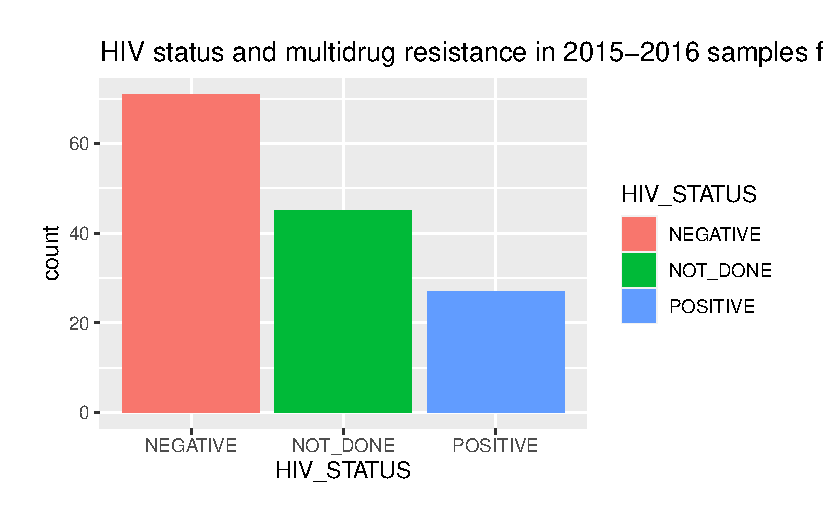
\includegraphics{MDR_TB_files/figure-pdf/unnamed-chunk-9-1.pdf}

}

\end{figure}

\hypertarget{tb-type-bar-plot}{%
\section{TB TYPE BAR PLOT}\label{tb-type-bar-plot}}

\begin{Shaded}
\begin{Highlighting}[]
\NormalTok{tb\_type\_bar }\OtherTok{\textless{}{-}} \FunctionTok{ggplot}\NormalTok{(mdr\_tb\_dfv1, }\AttributeTok{mapping =} \FunctionTok{aes}\NormalTok{(}\AttributeTok{x=}\NormalTok{TB\_TYPE)) }\SpecialCharTok{+} \FunctionTok{geom\_bar}\NormalTok{(}\AttributeTok{mapping =} \FunctionTok{aes}\NormalTok{(}\AttributeTok{fill =}\NormalTok{ TB\_TYPE)) }\SpecialCharTok{+} \FunctionTok{ggtitle}\NormalTok{(}\StringTok{\textquotesingle{}TB Type and multidrug resistance}
\StringTok{                                                                                                                 in 2015{-}2016 samples from NTRL\textquotesingle{}}\NormalTok{)}
\end{Highlighting}
\end{Shaded}

\hypertarget{smear-bar-plot}{%
\section{SMEAR BAR PLOT}\label{smear-bar-plot}}

\begin{Shaded}
\begin{Highlighting}[]
\NormalTok{smearBar }\OtherTok{\textless{}{-}} \FunctionTok{ggplot}\NormalTok{(mdr\_tb\_dfv1, }\AttributeTok{mapping =} \FunctionTok{aes}\NormalTok{(}\AttributeTok{x=}\NormalTok{SMEAR)) }\SpecialCharTok{+} \FunctionTok{geom\_bar}\NormalTok{(}\AttributeTok{mapping =} \FunctionTok{aes}\NormalTok{(}\AttributeTok{fill =}\NormalTok{ SMEAR)) }\SpecialCharTok{+} \FunctionTok{ggtitle}\NormalTok{(}\StringTok{\textquotesingle{}Smear results and multidrug resistance in 2015{-}2016 samples from NTRL\textquotesingle{}}\NormalTok{)}
\NormalTok{smearBar }
\end{Highlighting}
\end{Shaded}

\begin{figure}[H]

{\centering 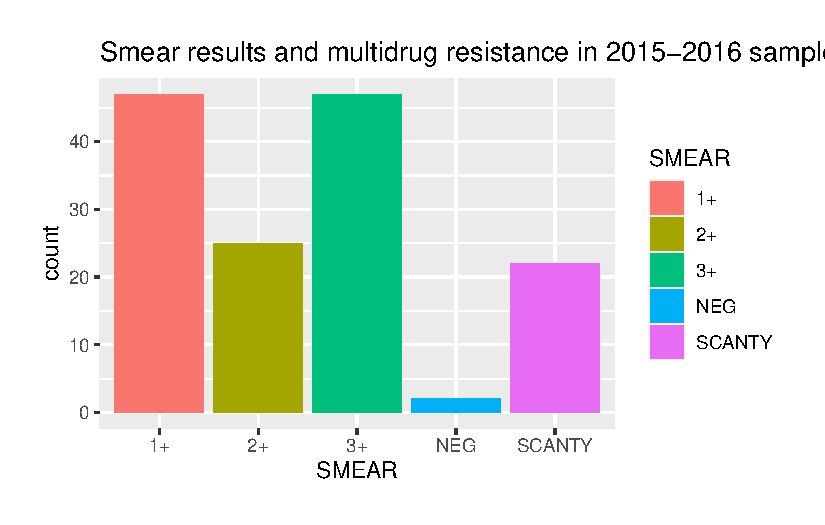
\includegraphics{MDR_TB_files/figure-pdf/unnamed-chunk-11-1.pdf}

}

\end{figure}

Age groups based on WHO typical age divisions

\begin{Shaded}
\begin{Highlighting}[]
\NormalTok{mdr\_tb\_dfv3 }\OtherTok{\textless{}{-}}\NormalTok{ mdr\_tb\_dfv1 }\SpecialCharTok{\%\textgreater{}\%}   \FunctionTok{mutate}\NormalTok{(}
  \CommentTok{\# Create categories}
  \AttributeTok{age\_group =}\NormalTok{ dplyr}\SpecialCharTok{::}\FunctionTok{case\_when}\NormalTok{(}
\NormalTok{    AGE }\SpecialCharTok{\textless{}=} \DecValTok{4}            \SpecialCharTok{\textasciitilde{}} \StringTok{"0{-}4"}\NormalTok{,}
\NormalTok{    AGE }\SpecialCharTok{\textgreater{}} \DecValTok{4} \SpecialCharTok{\&}\NormalTok{ AGE }\SpecialCharTok{\textless{}=} \DecValTok{14} \SpecialCharTok{\textasciitilde{}} \StringTok{"5{-}14"}\NormalTok{,}
\NormalTok{    AGE }\SpecialCharTok{\textgreater{}} \DecValTok{14} \SpecialCharTok{\&}\NormalTok{ AGE}\SpecialCharTok{\textless{}=} \DecValTok{24} \SpecialCharTok{\textasciitilde{}} \StringTok{"15{-}24"}\NormalTok{,}
\NormalTok{    AGE }\SpecialCharTok{\textgreater{}} \DecValTok{24} \SpecialCharTok{\&}\NormalTok{ AGE }\SpecialCharTok{\textless{}=} \DecValTok{34}  \SpecialCharTok{\textasciitilde{}} \StringTok{"25{-}34"}\NormalTok{,}
\NormalTok{    AGE }\SpecialCharTok{\textgreater{}} \DecValTok{34} \SpecialCharTok{\&}\NormalTok{ AGE }\SpecialCharTok{\textless{}=} \DecValTok{44} \SpecialCharTok{\textasciitilde{}} \StringTok{"35{-}44"}\NormalTok{,}
\NormalTok{    AGE }\SpecialCharTok{\textgreater{}} \DecValTok{44} \SpecialCharTok{\&}\NormalTok{ AGE }\SpecialCharTok{\textless{}=} \DecValTok{54} \SpecialCharTok{\textasciitilde{}} \StringTok{"45{-}54"}\NormalTok{,}
\NormalTok{    AGE }\SpecialCharTok{\textgreater{}} \DecValTok{54} \SpecialCharTok{\&}\NormalTok{ AGE }\SpecialCharTok{\textless{}=} \DecValTok{64} \SpecialCharTok{\textasciitilde{}} \StringTok{"65+"}\NormalTok{,}
\NormalTok{    AGE }\SpecialCharTok{\textgreater{}=} \DecValTok{64} \SpecialCharTok{\textasciitilde{}} \StringTok{"35{-}44"}
\NormalTok{  ),}
  \CommentTok{\# Convert to factor}
  \AttributeTok{age\_group =} \FunctionTok{factor}\NormalTok{(}
\NormalTok{    age\_group,}
    \AttributeTok{level =} \FunctionTok{c}\NormalTok{(}\StringTok{"0{-}4"}\NormalTok{, }\StringTok{"5{-}14"}\NormalTok{,}\StringTok{"15{-}24"}\NormalTok{,}\StringTok{"25{-}34"}\NormalTok{,}\StringTok{"35{-}44"}\NormalTok{,}\StringTok{"45{-}54"}\NormalTok{, }\StringTok{"65+"}\NormalTok{)}
\NormalTok{  )}
\NormalTok{)}
\end{Highlighting}
\end{Shaded}

\hypertarget{lollipop-plot-for-countygeographical-distribution}{%
\section{LOLLIPOP PLOT FOR COUNTY/GEOGRAPHICAL
DISTRIBUTION}\label{lollipop-plot-for-countygeographical-distribution}}

\begin{Shaded}
\begin{Highlighting}[]
\NormalTok{geoGrpsPcts }\OtherTok{\textless{}{-}} \FunctionTok{pcts}\NormalTok{(mdr\_tb\_dfv1, }\StringTok{\textquotesingle{}Province\textquotesingle{}}\NormalTok{)}

\NormalTok{GeoPops }\OtherTok{\textless{}{-}}\NormalTok{ geoGrpsPcts }\SpecialCharTok{\%\textgreater{}\%}

  \FunctionTok{arrange}\NormalTok{(}\FunctionTok{desc}\NormalTok{(Percentages)) }\SpecialCharTok{\%\textgreater{}\%} 

  \FunctionTok{mutate}\NormalTok{( }\AttributeTok{Province =}\NormalTok{ forcats}\SpecialCharTok{::}\FunctionTok{fct\_reorder}\NormalTok{(Province, Percentages)) }\SpecialCharTok{\%\textgreater{}\%}

  \FunctionTok{ggplot}\NormalTok{(}\FunctionTok{aes}\NormalTok{(}\AttributeTok{x=}\NormalTok{Province, }\AttributeTok{y=}\NormalTok{Percentages)) }\SpecialCharTok{+}

  \FunctionTok{geom\_point}\NormalTok{(}\AttributeTok{color =} \StringTok{\textquotesingle{}orange\textquotesingle{}}\NormalTok{) }\SpecialCharTok{+}

  \FunctionTok{geom\_segment}\NormalTok{(}\FunctionTok{aes}\NormalTok{(}\AttributeTok{x=}\NormalTok{Province, }\AttributeTok{y=}\NormalTok{Percentages, }\AttributeTok{xend=}\NormalTok{Province, }\AttributeTok{yend=}\DecValTok{0}\NormalTok{, }\AttributeTok{color =} \StringTok{\textquotesingle{}red\textquotesingle{}}\NormalTok{)) }\SpecialCharTok{+}

  \FunctionTok{theme}\NormalTok{(}\AttributeTok{axis.text.x =} \FunctionTok{element\_text}\NormalTok{(}\AttributeTok{angle =} \DecValTok{90}\NormalTok{), }\AttributeTok{panel.background =} \FunctionTok{element\_rect}\NormalTok{(}\AttributeTok{fill =} \StringTok{\textquotesingle{}lightblue\textquotesingle{}}\NormalTok{), }\AttributeTok{panel.grid.major =} \FunctionTok{element\_blank}\NormalTok{(), }\AttributeTok{panel.grid.minor =} \FunctionTok{element\_blank}\NormalTok{(), }\AttributeTok{plot.title =} \FunctionTok{element\_text}\NormalTok{(}\AttributeTok{color=}\StringTok{\textquotesingle{}\#6699CC\textquotesingle{}}\NormalTok{, }\AttributeTok{size =} \DecValTok{10}\NormalTok{, }\AttributeTok{face =} \StringTok{\textquotesingle{}bold\textquotesingle{}}\NormalTok{)) }\SpecialCharTok{+}

  \FunctionTok{labs}\NormalTok{(}\AttributeTok{title =} \StringTok{\textquotesingle{}MDR TB: Percentage of MDR TB cases by region/county reported to the NTRL\textquotesingle{}}\NormalTok{, }\AttributeTok{y=} \StringTok{\textquotesingle{}Percentage (\%) per county\textquotesingle{}}\NormalTok{, }\AttributeTok{x=}\StringTok{\textquotesingle{}County\textquotesingle{}}\NormalTok{) }\SpecialCharTok{+}

  \FunctionTok{guides}\NormalTok{(}\AttributeTok{color =} \StringTok{\textquotesingle{}none\textquotesingle{}}\NormalTok{)}
\NormalTok{GeoPops }
\end{Highlighting}
\end{Shaded}

\begin{figure}[H]

{\centering 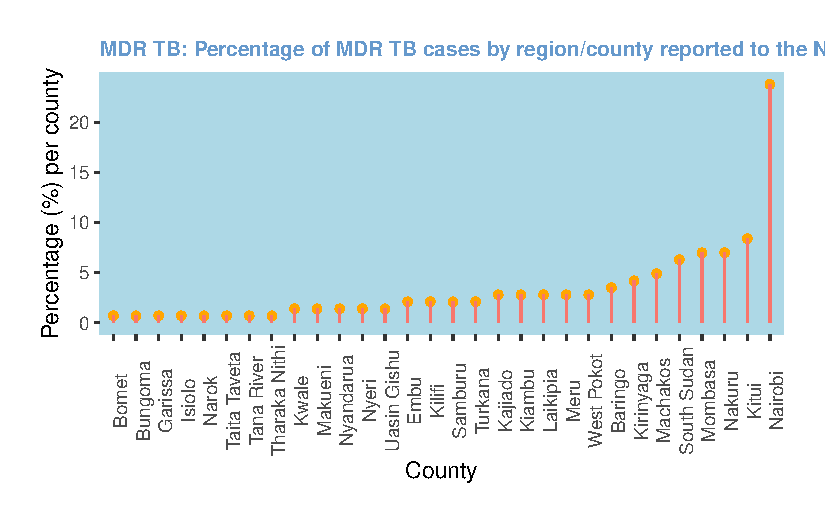
\includegraphics{MDR_TB_files/figure-pdf/unnamed-chunk-13-1.pdf}

}

\end{figure}

\hypertarget{age-group-bar-plot}{%
\section{AGE GROUP BAR PLOT}\label{age-group-bar-plot}}

\begin{Shaded}
\begin{Highlighting}[]
\NormalTok{age\_groupBars }\OtherTok{\textless{}{-}}\NormalTok{ mdr\_tb\_dfv3 }\SpecialCharTok{\%\textgreater{}\%}

  \FunctionTok{group\_by}\NormalTok{(age\_group) }\SpecialCharTok{\%\textgreater{}\%}

  \FunctionTok{summarise}\NormalTok{(}\AttributeTok{counts =} \FunctionTok{n}\NormalTok{())}

\FunctionTok{ggplot}\NormalTok{() }\SpecialCharTok{+}

  \FunctionTok{geom\_bar}\NormalTok{(}\AttributeTok{data =}\NormalTok{ age\_groupBars, }\FunctionTok{aes}\NormalTok{(}\AttributeTok{x =}\NormalTok{ age\_group, }\AttributeTok{y =}\NormalTok{ counts, }\AttributeTok{fill =}\NormalTok{ age\_group), }\AttributeTok{stat =} \StringTok{"identity"}\NormalTok{) }\SpecialCharTok{+}

  \FunctionTok{labs}\NormalTok{(}\AttributeTok{title =} \StringTok{\textquotesingle{}Age distribution of MDR isolates subitted to the NTRL between 2015{-}2015\textquotesingle{}}\NormalTok{)}
\end{Highlighting}
\end{Shaded}

\begin{figure}[H]

{\centering 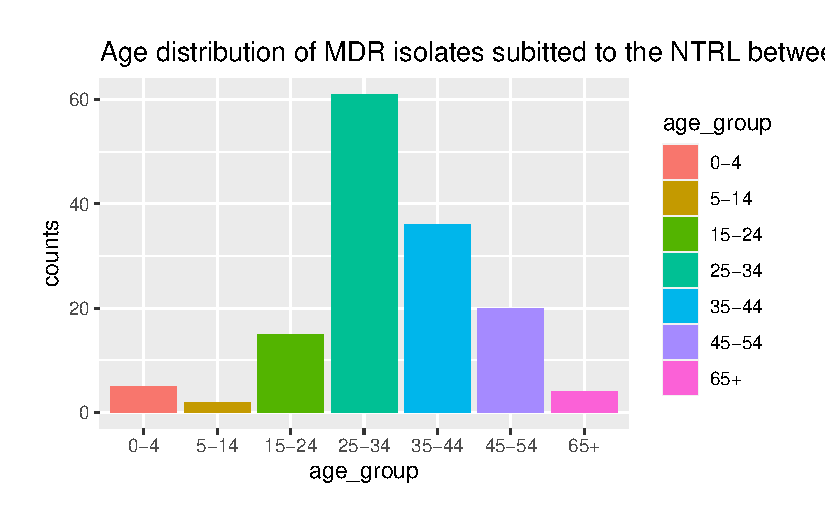
\includegraphics{MDR_TB_files/figure-pdf/unnamed-chunk-14-1.pdf}

}

\end{figure}

\begin{Shaded}
\begin{Highlighting}[]
\NormalTok{age\_groupBars}
\end{Highlighting}
\end{Shaded}

\begin{verbatim}
# A tibble: 7 x 2
  age_group counts
  <fct>      <int>
1 0-4            5
2 5-14           2
3 15-24         15
4 25-34         61
5 35-44         36
6 45-54         20
7 65+            4
\end{verbatim}

\hypertarget{inferential-statistics}{%
\chapter{\texorpdfstring{\textbf{INFERENTIAL
STATISTICS}}{INFERENTIAL STATISTICS}}\label{inferential-statistics}}

\hypertarget{fishers-exact-test-for-hiv-status}{%
\section{Fishers exact test for HIV
status}\label{fishers-exact-test-for-hiv-status}}

\begin{Shaded}
\begin{Highlighting}[]
\NormalTok{p\_value }\OtherTok{\textless{}{-}} \FunctionTok{Fishersfn}\NormalTok{(mdr\_tb\_dfv3, }\StringTok{\textquotesingle{}HIV\_STATUS\textquotesingle{}}\NormalTok{, }\StringTok{\textquotesingle{}MDR\_TYPE\textquotesingle{}}\NormalTok{)}
\NormalTok{p\_value }
\end{Highlighting}
\end{Shaded}

\begin{verbatim}

    Fisher's Exact Test for Count Data

data:  contingency_table
p-value = 0.2897
alternative hypothesis: two.sided
\end{verbatim}

\hypertarget{fishers-exact-test-for-age}{%
\section{Fisher's exact test for age}\label{fishers-exact-test-for-age}}

\begin{Shaded}
\begin{Highlighting}[]
\NormalTok{p\_value }\OtherTok{\textless{}{-}} \FunctionTok{Fishersfn}\NormalTok{(mdr\_tb\_dfv3, }\StringTok{\textquotesingle{}age\_group\textquotesingle{}}\NormalTok{, }\StringTok{\textquotesingle{}MDR\_TYPE\textquotesingle{}}\NormalTok{)}
\NormalTok{p\_value }
\end{Highlighting}
\end{Shaded}

\begin{verbatim}

    Fisher's Exact Test for Count Data

data:  contingency_table
p-value = 0.175
alternative hypothesis: two.sided
\end{verbatim}

\hypertarget{fishers-exact-test-for-county}{%
\section{Fisher's exact test for
COUNTY}\label{fishers-exact-test-for-county}}

\begin{Shaded}
\begin{Highlighting}[]
\NormalTok{p\_value }\OtherTok{\textless{}{-}} \FunctionTok{Fishersfn}\NormalTok{(mdr\_tb\_dfv1, }\StringTok{\textquotesingle{}Province\textquotesingle{}}\NormalTok{, }\StringTok{\textquotesingle{}MDR\_TYPE\textquotesingle{}}\NormalTok{)}
\NormalTok{p\_value}
\end{Highlighting}
\end{Shaded}

\begin{verbatim}

    Fisher's Exact Test for Count Data

data:  contingency_table
p-value = 0.06311
alternative hypothesis: two.sided
\end{verbatim}

\hypertarget{fishers-exact-test-for-tb-type}{%
\section{Fisher's exact test for TB
type}\label{fishers-exact-test-for-tb-type}}

\begin{Shaded}
\begin{Highlighting}[]
\NormalTok{p\_value }\OtherTok{\textless{}{-}} \FunctionTok{Fishersfn}\NormalTok{(mdr\_tb\_dfv1, }\StringTok{\textquotesingle{}TB\_TYPE\textquotesingle{}}\NormalTok{, }\StringTok{\textquotesingle{}MDR\_TYPE\textquotesingle{}}\NormalTok{)}
\NormalTok{p\_value}
\end{Highlighting}
\end{Shaded}

\begin{verbatim}

    Fisher's Exact Test for Count Data

data:  contingency_table
p-value = 0.9482
alternative hypothesis: two.sided
\end{verbatim}

\hypertarget{fishers-exact-test-for-gender}{%
\section{Fisher's exact test for
GENDER}\label{fishers-exact-test-for-gender}}

\begin{Shaded}
\begin{Highlighting}[]
\NormalTok{p\_value }\OtherTok{\textless{}{-}} \FunctionTok{Fishersfn}\NormalTok{(mdr\_tb\_dfv1, }\StringTok{\textquotesingle{}GENDER\textquotesingle{}}\NormalTok{, }\StringTok{\textquotesingle{}MDR\_TYPE\textquotesingle{}}\NormalTok{)}
\NormalTok{p\_value}
\end{Highlighting}
\end{Shaded}

\begin{verbatim}

    Fisher's Exact Test for Count Data

data:  contingency_table
p-value = 0.3319
alternative hypothesis: true odds ratio is not equal to 1
95 percent confidence interval:
 0.5015292 9.1443367
sample estimates:
odds ratio 
  2.088592 
\end{verbatim}

\hypertarget{fishers-exact-test-for-smears}{%
\section{Fisher's exact test for
SMEARS}\label{fishers-exact-test-for-smears}}

\begin{Shaded}
\begin{Highlighting}[]
\NormalTok{p\_value }\OtherTok{\textless{}{-}} \FunctionTok{Fishersfn}\NormalTok{(mdr\_tb\_dfv1, }\StringTok{\textquotesingle{}SMEAR\textquotesingle{}}\NormalTok{, }\StringTok{\textquotesingle{}MDR\_TYPE\textquotesingle{}}\NormalTok{)}
\NormalTok{p\_value}
\end{Highlighting}
\end{Shaded}

\begin{verbatim}

    Fisher's Exact Test for Count Data

data:  contingency_table
p-value = 0.7377
alternative hypothesis: two.sided
\end{verbatim}

\hypertarget{more-characterizations}{%
\chapter{More characterizations}\label{more-characterizations}}

\begin{Shaded}
\begin{Highlighting}[]
\NormalTok{mdr\_tb\_dfv5 }\OtherTok{\textless{}{-}}\NormalTok{ mdr\_tb\_df}\SpecialCharTok{$}\NormalTok{MDR\_TYPE[mdr\_tb\_df}\SpecialCharTok{$}\NormalTok{RpoB }\SpecialCharTok{==} \StringTok{\textquotesingle{}Resistant\textquotesingle{}} \SpecialCharTok{\&}\NormalTok{ mdr\_tb\_df}\SpecialCharTok{$}\NormalTok{KatG }\SpecialCharTok{==} \StringTok{\textquotesingle{}Resistant\textquotesingle{}} \SpecialCharTok{\&}\NormalTok{ mdr\_tb\_df}\SpecialCharTok{$}\NormalTok{inhA }\SpecialCharTok{==} \StringTok{\textquotesingle{}Resistant\textquotesingle{}}\NormalTok{] }\OtherTok{\textless{}{-}} \StringTok{\textquotesingle{}MDR+\textquotesingle{}}
\end{Highlighting}
\end{Shaded}

\hypertarget{percentages-of-the-mdr-types}{%
\chapter{Percentages of the MDR
types}\label{percentages-of-the-mdr-types}}

\begin{Shaded}
\begin{Highlighting}[]
\FunctionTok{pcts}\NormalTok{(mdr\_tb\_df, }\StringTok{\textquotesingle{}MDR\_TYPE\textquotesingle{}}\NormalTok{)}
\end{Highlighting}
\end{Shaded}

\begin{verbatim}
# A tibble: 3 x 3
  MDR_TYPE counts Percentages
  <chr>     <int>       <dbl>
1 MDR+          7        4.90
2 MDRIR        11        7.69
3 MDRKR       125       87.4 
\end{verbatim}

TABLES OF DEMOGRAPHIC DISTRIBUTION OF MDR TYPES

\begin{Shaded}
\begin{Highlighting}[]
\FunctionTok{table}\NormalTok{(mdr\_tb\_df}\SpecialCharTok{$}\NormalTok{Province, mdr\_tb\_df}\SpecialCharTok{$}\NormalTok{MDR\_TYPE)}
\end{Highlighting}
\end{Shaded}

\begin{verbatim}
               
                MDR+ MDRIR MDRKR
  Baringo          1     0     4
  Bomet            0     1     0
  Bungoma          0     0     1
  Embu             0     0     3
  Garissa          1     0     0
  Isiolo           0     0     1
  Kajiado          1     0     3
  Kiambu           0     0     4
  Kilifi           0     0     3
  Kirinyaga        0     1     5
  Kitui            0     1    11
  Kwale            0     0     2
  Laikipia         0     0     4
  Machakos         0     0     7
  Makueni          0     0     2
  Meru             1     1     2
  Mombasa          0     0    10
  Nairobi          2     1    31
  Nakuru           0     0    10
  Narok            0     0     1
  Nyandarua        0     0     2
  Nyeri            0     0     2
  Samburu          0     1     2
  South Sudan      1     2     6
  Taita Taveta     0     0     1
  Tana River       0     1     0
  Tharaka Nithi    0     0     1
  Turkana          0     0     3
  Uasin Gishu      0     1     1
  West Pokot       0     1     3
\end{verbatim}

\begin{Shaded}
\begin{Highlighting}[]
\FunctionTok{table}\NormalTok{(mdr\_tb\_df}\SpecialCharTok{$}\NormalTok{HIV\_STATUS, mdr\_tb\_df}\SpecialCharTok{$}\NormalTok{MDR\_TYPE)}
\end{Highlighting}
\end{Shaded}

\begin{verbatim}
          
           MDR+ MDRIR MDRKR
  NEGATIVE    2     3    66
  NOT_DONE    3     5    37
  POSITIVE    2     3    22
\end{verbatim}

\begin{Shaded}
\begin{Highlighting}[]
\FunctionTok{table}\NormalTok{(mdr\_tb\_df}\SpecialCharTok{$}\NormalTok{SMEAR, mdr\_tb\_df}\SpecialCharTok{$}\NormalTok{MDR\_TYPE)}
\end{Highlighting}
\end{Shaded}

\begin{verbatim}
        
         MDR+ MDRIR MDRKR
  1+        2     5    40
  2+        2     2    21
  3+        1     2    44
  NEG       1     0     1
  SCANTY    1     2    19
\end{verbatim}

\begin{Shaded}
\begin{Highlighting}[]
\FunctionTok{table}\NormalTok{(mdr\_tb\_df}\SpecialCharTok{$}\NormalTok{TB\_TYPE, mdr\_tb\_df}\SpecialCharTok{$}\NormalTok{MDR\_TYPE)}
\end{Highlighting}
\end{Shaded}

\begin{verbatim}
            
             MDR+ MDRIR MDRKR
  FA_1STL_TR    1     3    31
  FA_RE_TREA    0     0     3
  MDR_CONTA     0     0     3
  MDR_F         1     1    22
  NEW           1     4    26
  RE_AF_DEFA    0     1    13
  SP_SM_NR      0     0     3
  SP_SM_PR      4     2    23
  UNKNOWN       0     0     1
\end{verbatim}



\end{document}
